%-----------------------------------------------
% Template para criação de resumos de projectos/dissertação
% jlopes AT fe.up.pt,   Fri Jul  3 11:08:59 2009
%-----------------------------------------------

\documentclass[9pt,a4paper]{extarticle}

%% English version: comment first, uncomment second
%\usepackage[portuguese]{babel}  % Portuguese
\usepackage[english]{babel}     % English
\usepackage{graphicx}           % images .png or .pdf w/ pdflatex OR .eps w/ latex
\usepackage{times}              % use Times type-1 fonts
\usepackage[utf8]{inputenc}     % 8 bits using UTF-8
\usepackage{url}                % URLs
\usepackage{multicol}           % twocolumn, etc
\usepackage{float}              % improve figures & tables floating
\usepackage[tableposition=top]{caption} % captions
%% English version: comment first (maybe)
%\usepackage{indentfirst}        % portuguese standard for paragraphs
%\usepackage{parskip}

%% page layout
\usepackage[a4paper,margin=30mm,noheadfoot]{geometry}

\usepackage{multirow}

%% space between columns
\columnsep 12mm

%% headers & footers
\pagestyle{empty}

%% figure & table caption
\captionsetup{figurename=Fig.,tablename=Tab.,labelsep=endash,font=bf,skip=.5\baselineskip}

%% heading
\makeatletter
\renewcommand*{\@seccntformat}[1]{%
  \csname the#1\endcsname.\quad
}
\makeatother

%% avoid widows and orphans
\clubpenalty=300
\widowpenalty=300

\begin{document}

\title{\vspace*{-8mm}\textbf{\textsc{Estudo, conceção, desenvolvimento e teste de uma aplicação móvel de pagamento e validação para Transportes Públicos de Passageiros}}}
\author{\emph{André Gonçalves Dias}\\[2mm]
\small{Project/Dissertation under orientation of \emph{Prof.\ João Bernardo de Sena Esteves Falcão e Cunha} and \emph{Prof.\ Marta Maria Campos Ferreira}}}
\date{}
\maketitle
%no page number 
\thispagestyle{empty}

\vspace*{-4mm}\noindent\rule{\textwidth}{0.4pt}\vspace*{4mm}

\begin{multicols}{2}

\section{Motivation}\label{sec:motiva}

The aim of this project is to ease the payment and validation of travel tickets in public transportation of the Porto Metropolitan Area, taking advantage of mobile devices. On the other side, it aims to solve the problem caused by forgetting or losing the card that, in many cases, leads to the need of buying a new card and travel tickets. In the case of losing it, it also leads to the impossibility of using the stored tickets.
\\The main motivation of this work is the high number of passengers that travel by public transportation in the Porto Metropolitan Area. Throughout 2012, fifty four and a half million passengers travelled by Metro \cite{INE20130528} and forty five million passengers by bus (referring to the intermodal system validations) in the first semester of 2012. \cite{andante}
\\If the high number of passengers serves as a base for the development theme choice, the chosen technology is based in the fact that one in each five people already uses Internet services on their mobile phone \cite{INE20121106}, and also that it’s less and less probable to forget the mobile phone at home. A study shows that people are more likely to forget the wallet at home than the mobile phone. \cite{NFCForum2011}.
\\The possibility to add value to the already existing services is also a great motivation for the project development.

\section{Objectives}\label{sec:goals}

The objectives of this project are:
\begin{itemize}
\item To create a new way of payment and validation of travel tickets, not replacing the actual model, but serving as a complement;
\item To reduce the queues in the Andante stores and automatic vending machines, decentralizing the operation of buying that, many times, causes long waiting periods, especially in the beginning or ending of the month, caused by the monthly signature renewal;
\item To reduce production and maintenance costs of cards, as there is no need to have a physical card, everything is stored in the passenger’s mobile device;
\item To provide statistical information about passengers to public transportation operators, allowing them to better adjust and plan the routes and distribution of vehicles;
\item To allow multiple operations anywhere and through a single channel, providing a set of services at the distance of one click, dropping the need to check information in the information boards, buy tickets in an automatic vending machine or Andante store and validate the ticket in the specially designed machines;
\item To increase the overall satisfaction of users, bringing them more commodity and providing them a service that allows them to save time and energy.
\end{itemize}


\section{Work Description}\label{sec:work}

The objective of this project is to drop the need of a physical element (card) in the payment and validation operations in the public transportation system of the Porto Metropolitan Area, with the implementation of a remote payment and validation system via Internet, using mobile devices with Android operating system. Besides that, the gathering of information related to the main infrastructures used in this purpose, studying the main features and operations needed in the application and developing appropriate solutions for the existing problems are also important in this project.
\\As main functional requirements, this system has to provide a way of charging the virtual wallet, buying and validating (entry and exit (optional)) of travel tickets and verifying validity by an authorized conductor; the usual requirements of a traditional public transportation system. \cite{Buttyan2009}
\\In the future, it’s expected that this project is integrated with the MOVE-ME application, already available, serving as an add-on with new features and also providing the system administrator information related to passengers’ travels.

\subsection{Architecture}

The system is composed of three fundamental components. The \textbf{Server} component, posing as the centre of the system since it provides the various services that the other components interact with. The \textbf{Client} component, that allows the passenger to remotely access the available services. Finally, the \textbf{Conductor} component, which allows conductors to check passengers’ validity (those who use the system). In this phase, these two last components are built in the same application, in the passenger mobile device, dropping the need of providing the conductors special devices. 
\\This architecture follows the traditional Server-Client architecture, as shown in the Figure~\ref{fig:architecture}.

\begin{figure}[H]
\centerline{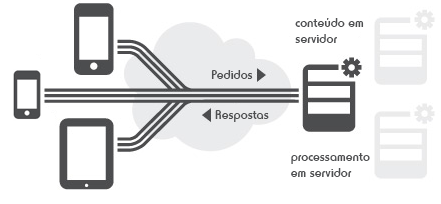
\includegraphics[scale=0.45]{architecture}}
    \caption{Arquitetura Servidor-Cliente}
    \label{fig:architecture}
\end{figure}

\subsection{Android}

Android was the operative system chosen because it’s the most popular mobile platform in the world. With an Android device, users can access all Google services that they are used to, and also more than 600 thousand applications and games available in the virtual store Google Play, many of those for free. Besides that, it’s possible to obtain millions of songs and books and thousands of movies. Android devices are constantly being updated and improved, gaining new and better features. It also provides users with a unique and custom experience.
\\The fact that the MOVE-ME application is already developed for this system is very important, easing the integration of both.
\\The chosen base version is 2.2 (Froyo), since more than 98\% of devices have this version or higher and it offers the required features. \cite{dashboards}

\section{Conclusions}\label{sec:conclui}

The fact that more and more public transportation passengers are owners of mobile devices, constantly consuming information, opens the doors for mobile ticketing, without any barriers. The users were very satisfied with the commodity and simplicity of the concept.
\\Another advantage of this system comparing to others in the same field, is the removal of every physical infrastructure throughout all the usage process. All the operations are done through mobile devices. However, this system takes advantage of the open system implemented in the Porto Metropolitan Area. It’s not possible to use it in a closed (with barriers) system without making the proper adaptations.

~\\In a general conclusion, the concept is approved, it’s practicable, and now it needs to be strengthened and simplified in order to be used by all the public transportation operators of the Porto Metropolitan Area, bringing them additional information about their passengers and providing users a practical, comfortable and effective solution for their travels.

%%English version: comment first, uncomment second
%\bibliographystyle{unsrt-pt}  % numeric, unsorted refs
\bibliographystyle{unsrt}  % numeric, unsorted refs
\bibliography{refs}

\end{multicols}

\end{document}
